\chapter{Cross-lingual Word Embedding without Parallel Data}

Learning a good mapping still need seed word translation pairs as cross-lingual supervision signals. For example in the first work use five thousand seeds to train the linear mapping. \cite{vulic2016role} shows that a seed dictionary of at least hundreds are need for the model to generalize.
\cite{zhang2017adversarial} proposed an adversarial autoencoder, using the generator $G$ to implement the mapping so that the transformed source embedding similar to the corresponding target embedding, and the discriminator $D$ strives to distinguish the target embedding from the transformed source embedding. \cite{conneau2017word} simplifies the structure


However, large dictionary is also not readily available for many language pairs.

Several unsupervised learning algorithms are studies   




\begin{figure}[t]
	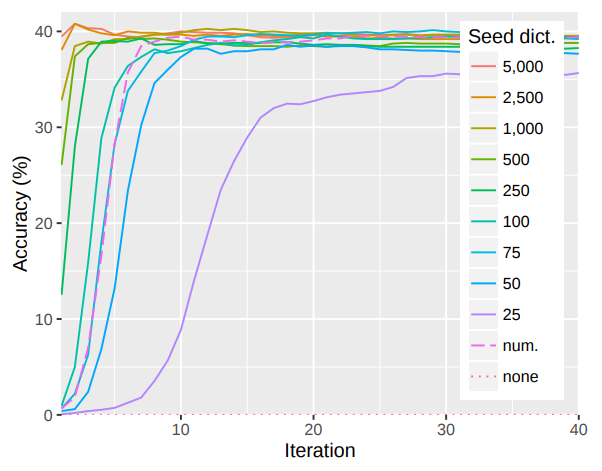
\includegraphics[width=12cm]{iter1}
	\centering
	\caption{Accuracy on bilingual lexicon induction}
\end{figure}	







\section{Initialization}
\cite{artetxe2018robust}.\\As it can be clearly observed that, the self learning algorithm can effectively learn the mapping between the source and target distribution even starts with a small dictionary size and the final accuracy when the algorithm converges are nearly the same level. However when start randomly without any support of dictionary, the framework does not work. In order to realize a fully unsupervised learning, we need to design heuristics to build the seed dictionary.

For total unsupervised learning, there is no direct alignment between the languages. 	The most challenge for unsupervised learning is the initialization. As proved in the experiment of \cite{}, the self-learning framework can work even with a small dictionary set, however the model cannot work without such dictionary as hint.  So it is important to find heuristic methods to initialize the model.

Several models are proposed:
Based on matrices ${M_E = EE^T}$, ${M_F = FF^T}$, we can exploit latent information to reduce the mismatch. Assume that, the words in the source and target set are most common. For a specific word, the corresponding line in ${M_E}$ demonstrates the distribution of similarity in the source vocabulary. ${M_E}$, ${M_F}$ can be nearly equivalent up to a permutation of the words. 
Instead of explore all the probability of permutation, he first sorts the values in each row of ${M_F}$ and ${M_E}$

Assume the SVD of ${E = USV^T}$,  the similarity ${M_E = US^2U^T}$. In practice, he computed sorted ${1}$, ${2}$	yielding the matrix ${E^{\prime}}$ , ${F^{\prime}}$ and used to build the initial solution for self-learning.

\subsection{Heuristics}
\subsubsection{Iterative Closest Point Method}
Assume that many language pairs share same principle axes of variation. We do the approximate distribution alignment with PCA.
For each language, we first select most frequent word vector,center the data and project it to the top ${p}$ principle components. We denote the projected language representation as 	${P_l \in {R}^{N * p}}$
Propose a method first learn ${T_{ef}}$ and ${T_{fe}}$ for ${E \rightarrow F}$ and ${F \rightarrow E}$ , we include the cycle-constraints ensure that a word ${f}$ transformed into joint embedding space and transformed back is unchanged. 


\begin{enumerate}
	\item For each ${e_i}$, find the nearest ${W_{fe} f_j}$.  denote as ${f(e_i)}$
	\item For each ${f_j}$, find the nearest ${W_{ef} e_i}$, denote as ${e(f_j)}$
	\item For all mini-barches of ${e_i}$ and ${f_j}$ in epoch, iterative optimize ${T_{ef}}$ and ${T_{fe}}$ on: \\
	${ \sum_{i} {\lVert e_i - W_{fe} f(e_i)\rVert} + \sum_j {\rVert f_j - W_{ef} e(f_j)\rVert} + \lambda {\sum_i}{\lVert e_i- W_{fe} W_{ef} e_i \rVert}  +  \lambda \sum_j {\lVert f_j - W_{ef} W_{fe} f_j \rVert}}$
\end{enumerate}
\subsection{Adversarial autoencoder}
The intuition can be formalized as the minimax game with the value function:
\begin{align*}
	V(D, G) = & E_{e\sim {p_e}}[\log D(e)] + E_{f \sim {p_f}} [\log (1-D(G(f)))]
\end{align*}
As a generic binary classifier, a feed-forward neural network with one hidden layer is used to parameterize the discriminator $D$, and its loss function is the usual cross-entropy loss.
\[L_D = -\log D(f) - \log (1-D(G(e)))\]
After the generator $G$ transforms a source word embedding $e$ into a target language representation $Gf$, we should be able to reconstruct the source word embedding $f$ by mapping back with $G^T$. We therefore introduce the reconstruction loss measured by cosine similarity:
\[ L_R = -\cos (f, G^TG))\]
Note that this loss will be minimized if $G$ is orthogonal. With this term included, the loss function for the generator becomes
\[ L_G = -\log D(G(x)) - \lambda \cos(f, G^TGf)\]
where $\lambda$ is a hyper-parameter that balances the two terms. 
\subsection{Adversarial Training}
Discriminator is trained to discriminate between elements randomly sampled from ${Wf_i}$ and ${e_j}$ and generator ${W}$ is trained to prevent the discriminator from making accurate prediction\\

The training algorithm follows the standard procedure of deep adversarial networks(GAN) of Goodfellow \cite{bibid}: the discriminator and generator are trained iteratively with the stochastic gradient descent to minimize the ${L_D}$ and ${L_w}$

Let ${=\{ x_1, \cdots, x_n\}}$ and ${ = \{ y_i, \cdots , y_m\}}$ be the two sets of $n$ and $m$ word embeddings from a source and a target language separately, We refer the discriminator parameters as ${\theta_D}$.The discriminator is a multi-layer neural network trained to discriminate the transformed source word embedding from the target word embedding, while the mapping $W$, simply a linear transformation, is trained to fooling discriminator. In the two-player game, we are supposed to learn the mapping from source embedding space to the target space.
Discriminator objective  
\[ L_D(\theta_D | W) =  -\frac{1}{n} \sum_{i=1}^{n} \log P_{\theta_D}(source = 1| Wf_i) - \frac{1}{m} \sum_{i=1}^{m} \log P_{\theta_D}(source=0| e_i) \]	

Mapping objective 
\[ L_W(W|\theta_D) =  -\frac{1}{n} \sum_{i=1}^{n}\log P_{\theta_D}(source=0|W f_i) - \frac{1}{m} \sum_{i=1}^{m} \log P_{\theta_D}(source = 1 | e_i) \]

\subsubsection{Model Selection}
Since the cross-lingual embedding training is under the unsupervised setting, We do not know the word translation accuracy, otherwise if we have the validation data, that means we will have parallel data, against the unsupervised idea. To address this issue, we must select from the property of data or the loss of the neural network as the unsupervised criterion. However in the experiments we find that the accuracy of the discriminator always stays at a high level no matter how is the word translation accuracy. 

All these methods can be use to find meaningful word pairs in both languages. For further refinement we can use the induced dictionary to start the iterative self-learning algorithm. 
\section{Iterative Training}
\subsection{Self-learning with Procrustes}
Self-learning framework\\

\begin{figure}[ht]
	\centering
	\begin{minipage}{.7\linewidth}
		\begin{algorithm}[H]
			\SetAlgoLined
			\KwIn{$\mathcal{F}$ (source embeddings)}
			\KwIn{$\mathcal{E}$ (target embeddings)}
			\KwIn{$\mathcal{D}$ (seed dictionary)}
			\KwResult{$\mathcal{W}$ (embedding mapping) }
			\While{not converge}{
				${\mathcal{W} \leftarrow LEARN\_MAPPING(\mathcal{F},\mathcal{E},\mathcal{D})}$
				${\mathcal{D} \leftarrow LEARN\_DICTIONARY}$
				
			}
			
			\caption{Self-learning framework}
		\end{algorithm}
	\end{minipage}
\end{figure}


\begin{figure}[t]
	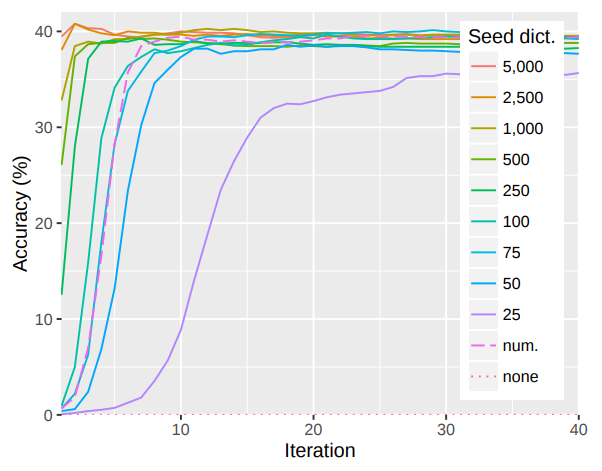
\includegraphics[width=12cm]{iter1}
	\centering
	\caption{Accuracy on bilingual lexicon induction}
\end{figure}
\subsection{Data-driven Method}
Training procedure:
\begin{enumerate}
	\item translate corpus according to current mapping, get the word pairs $D$
	\item train the network with $D$ to minimize the mapping distance
	\item Repeat $1,2$ until the algorithm converges
\end{enumerate}
		\[ 
		\left. \begin{array}{c c} 
		(f_1,& e_1)\\
		(f_2,& e_2)\\
		\multicolumn{2}{c}{\vdots}\\
		(f_N,& e_N)
		\end{array} \right\} 
		\Rightarrow D
		\]

		\[\mathcal{L} = \sum_{(f,e)\in D} {\lVert Wf - e \rVert}^2  \]

\section{Word Translation Induction}
The CSLS as described by \cite{conneau2017word}, can be written as:
\[ CSLS(\bm{e}, \bm{f}) = 2 cos(\bm{e}, \bm{y}) - \frac{1}{K} \sum_{\bm{e^{\prime}} \in N(\bm{e})} cos(\bm{f}, \bm{e^{\prime}})- \frac{1}{K} \sum_{\bm{f^{\prime}} \in N(\bm{e})} cos(\bm{f^{\prime}}, \bm{e}) \]
Since the embedding space is of high dimension and the nearest neighbour search is performed here, so that a few embeddings embedding will become the nearest neighbour of many data pointsto The obtained is known to suffer from the hubness problem, 
We denote ${N_Y(x)}$ the set of ${K}$ nearest neighbors of points in the target embedding space, and ${N_X(y)}$ the nearest neighbors of ${y}$ in the source embedding space. 
So in this way we penalize the hub points
A good initialization is import for ICP methods, so begin with the projected data, and initialize transformation ${T_{ef}}$ and ${T_{fe}}$ with the identity matrix.
After several iterations of, the estimated transformation becomes quite reliable.  Then use this transformation to find the matches.

\section{Non-linear Mapping}
